% =============================================
% VisionLab — Présentation Beamer
% Université de Yaoundé 1 — Faculté des Sciences
% Département d'Informatique — Licence 3
% =============================================
\documentclass[aspectratio=169, 11pt]{beamer}

% — Thème et couleurs ——————————————————————————
\usetheme{Madrid}
\usecolortheme{seahorse}
\definecolor{uy1blue}{RGB}{0, 82, 155}
\definecolor{uy1dark}{RGB}{20, 30, 48}
\definecolor{uy1accent}{RGB}{59, 130, 246}
\definecolor{uy1green}{RGB}{34, 197, 94}
\definecolor{uy1purple}{RGB}{139, 92, 246}

\setbeamercolor{palette primary}{bg=uy1blue, fg=white}
\setbeamercolor{palette secondary}{bg=uy1dark, fg=white}
\setbeamercolor{palette tertiary}{bg=uy1accent, fg=white}
\setbeamercolor{frametitle}{bg=uy1blue, fg=white}
\setbeamercolor{title}{fg=uy1blue}
\setbeamercolor{block title}{bg=uy1blue, fg=white}
\setbeamercolor{block body}{bg=uy1blue!5}
\setbeamercolor{block title alerted}{bg=red!80!black, fg=white}
\setbeamercolor{block title example}{bg=uy1green!80!black, fg=white}
\setbeamercolor{item}{fg=uy1blue}

\setbeamertemplate{navigation symbols}{}
\setbeamertemplate{footline}{
  \leavevmode\hbox{%
    \begin{beamercolorbox}[wd=.33\paperwidth,ht=2.5ex,dp=1ex,center]{palette primary}
      \usebeamerfont{author in head/foot}\insertshortauthor
    \end{beamercolorbox}%
    \begin{beamercolorbox}[wd=.34\paperwidth,ht=2.5ex,dp=1ex,center]{palette secondary}
      \usebeamerfont{title in head/foot}\insertshorttitle
    \end{beamercolorbox}%
    \begin{beamercolorbox}[wd=.33\paperwidth,ht=2.5ex,dp=1ex,right]{palette primary}
      \insertframenumber{} / \inserttotalframenumber\hspace*{2ex}
    \end{beamercolorbox}%
  }
}

% — Packages ———————————————————————————————————
\usepackage[utf8]{inputenc}
\usepackage[T1]{fontenc}
\usepackage[french]{babel}
\usepackage{graphicx}
\usepackage{amsmath, amssymb}
\usepackage{booktabs}
\usepackage{multicol}
\usepackage{tikz}
\usepackage{hyperref}
\usepackage{listings}
\usepackage{xcolor}
\usepackage{fancybox}

\graphicspath{{images/}}

\lstset{
  language=Java,
  basicstyle=\ttfamily\tiny,
  keywordstyle=\color{uy1blue}\bfseries,
  commentstyle=\color{gray},
  stringstyle=\color{uy1green},
  breaklines=true,
  frame=single,
  rulecolor=\color{uy1blue!30},
  backgroundcolor=\color{uy1blue!3},
}

% — Informations ———————————————————————————————
\title[VisionLab]{%
  \textbf{VisionLab}\\[4pt]
  \small Studio Interactif de Traitement d'Images Numériques}
\subtitle{Projet de Traitement d'Images — Licence 3 Informatique}
\author[N. Nassaramadji]{%
  \textbf{NASSARAMADJI Nasaire}\\[2pt]
  {\footnotesize Sous la supervision de \textbf{Pr TAPAMO KENFACK Hippolyte}}}
\institute[UY1]{%
  Université de Yaoundé~1\\
  Faculté des Sciences — Département d'Informatique}
\date{Année Académique 2025 — 2026}

% Logo UY1 (remplacez par le vrai logo si disponible)
% \titlegraphic{\includegraphics[height=1.2cm]{images/logo_uy1.png}}

% ==============================================
\begin{document}

% --- Page de Titre ---
\begin{frame}[plain]
  \vfill
  \begin{center}
    \begin{tikzpicture}
      \fill[uy1blue!10, rounded corners=10pt] (-7,-3.5) rectangle (7,3.5);
      \node at (0,2.2) {\Large\textbf{\textcolor{uy1blue}{UNIVERSITÉ DE YAOUNDÉ~1}}};
      \node at (0,1.6) {\small\textcolor{uy1dark}{Faculté des Sciences — Département d'Informatique}};
      \draw[uy1blue, thick] (-5,1.2) -- (5,1.2);
      \node at (0,0.4) {\LARGE\textbf{\textcolor{uy1dark}{VisionLab}}};
      \node at (0,-0.3) {\normalsize\textcolor{uy1blue}{Studio Interactif de Traitement d'Images Numériques}};
      \draw[uy1accent, thick] (-3,-0.7) -- (3,-0.7);
      \node at (0,-1.4) {\small\textcolor{uy1dark}{Présenté par : \textbf{NASSARAMADJI Nasaire}}};
      \node at (0,-2.0) {\small\textcolor{uy1dark}{Superviseur : \textbf{Pr TAPAMO KENFACK Hippolyte}}};
      \node at (0,-2.8) {\footnotesize\textcolor{gray}{Licence 3 Informatique — Année Académique 2025–2026}};
    \end{tikzpicture}
  \end{center}
  \vfill
\end{frame}

% --- Sommaire ---
\begin{frame}{Sommaire}
  \tableofcontents[hideallsubsections]
\end{frame}

% ======================================================================
\section{Introduction}
% ======================================================================

\begin{frame}{Contexte et Motivation}
  \begin{columns}[T]
    \column{0.55\textwidth}
    \begin{block}{Contexte}
      Le traitement d'images numériques est au cœur de nombreuses applications modernes :
      \begin{itemize}
        \item Imagerie médicale (IRM, Scanner)
        \item Reconnaissance de formes
        \item Télédétection et cartographie
        \item Véhicules autonomes
      \end{itemize}
    \end{block}
    \vspace{6pt}
    \begin{alertblock}{Problématique}
      Comment offrir une plateforme \textbf{interactive} et \textbf{accessible} permettant d'explorer les algorithmes fondamentaux du traitement d'images?
    \end{alertblock}

    \column{0.42\textwidth}
    % ► CAPTURE : Page d'accueil du studio (zone d'upload)
    % \includegraphics[width=\linewidth]{capture_accueil.png}
    \begin{tikzpicture}
      \fill[uy1blue!8, rounded corners=6pt] (0,0) rectangle (5,3.5);
      \node[text=uy1blue, font=\footnotesize\bfseries] at (2.5,2.8) {CAPTURE D'ÉCRAN};
      \node[text=gray, font=\scriptsize, text width=4cm, align=center] at (2.5,1.5) {Page d'accueil du studio\\(Zone d'importation)\\[6pt]\texttt{capture\_accueil.png}};
    \end{tikzpicture}
  \end{columns}
\end{frame}

\begin{frame}{Objectifs du Projet}
  \begin{exampleblock}{Objectif Général}
    Concevoir et développer une application web de traitement d'images implémentant les 6 chapitres du cours de \textbf{Traitement d'Images} de Licence~3.
  \end{exampleblock}
  \vspace{8pt}
  \begin{columns}[T]
    \column{0.48\textwidth}
    \textbf{\textcolor{uy1blue}{Objectifs Spécifiques :}}
    \begin{enumerate}
      \item Implémenter les transformations de base (luminosité, contraste, histogramme)
      \item Réaliser le filtrage spatial par convolution
      \item Développer l'analyse fréquentielle (FFT~2D)
      \item Coder la détection de contours multi-opérateurs
      \item Intégrer la segmentation par seuillage (Otsu)
      \item Appliquer la morphologie mathématique
    \end{enumerate}

    \column{0.48\textwidth}
    \textbf{\textcolor{uy1purple}{Stack Technologique :}}
    \begin{itemize}
      \item \textbf{Frontend} : React~19 + Vite~8
      \item \textbf{Style} : Tailwind~CSS~4
      \item \textbf{Icônes} : Lucide React
      \item \textbf{Algorithmique} : JavaScript natif
      \item \textbf{Rendu} : Canvas~2D API
      \item \textbf{Déploiement} : Render + GitHub
    \end{itemize}
    \vspace{6pt}
    \begin{center}
      \footnotesize\textcolor{gray}{\url{https://visionlab.nb-mind.com}}
    \end{center}
  \end{columns}
\end{frame}

% ======================================================================
\section{Architecture de l'Application}
% ======================================================================

\begin{frame}{Architecture Générale}
  \begin{center}
    \begin{tikzpicture}[
      box/.style={draw=uy1blue, fill=uy1blue!8, rounded corners=4pt,
                  minimum width=2.8cm, minimum height=1cm, font=\footnotesize\bfseries, align=center},
      arrow/.style={->, thick, uy1blue},
      scale=0.95, transform shape
    ]
      % Utilisateur
      \node[box, fill=uy1green!15, draw=uy1green!60] (user) at (0,0) {Utilisateur\\(Navigateur)};

      % Frontend
      \node[box] (app) at (4,0) {App.jsx\\(Routeur)};
      \node[box] (studio) at (8,1) {Studio.jsx\\(Page Studio)};
      \node[box] (support) at (8,-1) {Support.jsx\\(Page Support)};

      % Composants
      \node[box, fill=uy1accent!10] (sidebar) at (12,2) {Sidebar};
      \node[box, fill=uy1accent!10] (workspace) at (12,0.5) {ImageWorkspace};
      \node[box, fill=uy1accent!10] (control) at (12,-0.8) {ControlPanel};

      % Algorithmes
      \node[box, fill=uy1purple!12, draw=uy1purple!50] (algo) at (12,-2.5) {imageAlgorithms.js\\imageProcessing.js};

      % Flèches
      \draw[arrow] (user) -- (app);
      \draw[arrow] (app) -- (studio);
      \draw[arrow] (app) -- (support);
      \draw[arrow] (studio) -- (sidebar);
      \draw[arrow] (studio) -- (workspace);
      \draw[arrow] (studio) -- (control);
      \draw[arrow, uy1purple] (workspace) -- (algo);
      \draw[arrow, uy1purple, dashed] (control) -- (algo);
    \end{tikzpicture}
  \end{center}
  \vspace{4pt}
  \begin{center}
    \footnotesize\textcolor{gray}{Architecture modulaire : chaque chapitre correspond à un module activable dans le panneau de contrôle.}
  \end{center}
\end{frame}

\begin{frame}{Pipeline de Traitement}
  \begin{center}
    \begin{tikzpicture}[
      step/.style={draw=uy1blue, fill=white, rounded corners=3pt,
                   minimum width=2cm, minimum height=0.8cm, font=\tiny\bfseries, align=center},
      arr/.style={->, thick, uy1accent},
      scale=0.88, transform shape
    ]
      \node[step] (s1) at (0,0) {Image\\Originale};
      \node[step] (s2) at (2.5,0) {Niveaux\\de Gris};
      \node[step] (s3) at (5,0) {Interpolation\\(Ch.1)};
      \node[step] (s4) at (7.5,0) {Transf. de\\Base (Ch.1)};
      \node[step] (s5) at (10,0) {Convolution\\(Ch.2)};
      \node[step] (s6) at (12.5,0) {FFT\\(Ch.3)};
      \node[step] (s7) at (2.5,-1.5) {Contours\\(Ch.4)};
      \node[step] (s8) at (5,-1.5) {Segmentation\\(Ch.5)};
      \node[step] (s9) at (7.5,-1.5) {Morphologie\\(Ch.6)};
      \node[step, fill=uy1green!15, draw=uy1green] (s10) at (10.5,-1.5) {Image\\Résultat};

      \draw[arr] (s1) -- (s2);
      \draw[arr] (s2) -- (s3);
      \draw[arr] (s3) -- (s4);
      \draw[arr] (s4) -- (s5);
      \draw[arr] (s5) -- (s6);
      \draw[arr] (s6.south) |- (s7.east);
      \draw[arr] (s7) -- (s8);
      \draw[arr] (s8) -- (s9);
      \draw[arr] (s9) -- (s10);
    \end{tikzpicture}
  \end{center}
  \vspace{6pt}
  \begin{block}{Fonction centrale : \texttt{applyAllFilters()}}
    Cette fonction orchestre l'ensemble du pipeline dans \texttt{ImageWorkspace.jsx}.
    Chaque étape est conditionnée par l'objet \texttt{config} mis à jour depuis le \texttt{ControlPanel}.
  \end{block}
\end{frame}

% ======================================================================
\section{Chapitre 1 — Traitement de Base}
% ======================================================================

\begin{frame}{Chapitre 1 : Traitement de Base}
  \begin{columns}[T]
    \column{0.52\textwidth}
    \textbf{\textcolor{uy1blue}{Fonctionnalités implémentées :}}
    \begin{itemize}
      \item \textbf{Luminosité} : $g(x,y) = f(x,y) + \beta$
      \item \textbf{Contraste} : $g(x,y) = \alpha \cdot f(x,y)$
      \item \textbf{Égalisation d'histogramme} :
        \[ h(v) = \text{round}\left(\frac{(L-1)}{M \times N} \sum_{j=0}^{v} n_j \right) \]
      \item \textbf{Opérations arithmétiques} : Addition, soustraction, multiplication de deux images
      \item \textbf{Interpolation} :
        \begin{itemize}
          \item Plus Proche Voisin
          \item Bilinéaire
        \end{itemize}
    \end{itemize}

    \column{0.45\textwidth}
    % ► CAPTURE : Chapitre 1 avec curseurs luminosité/contraste et histogramme
    % \includegraphics[width=\linewidth]{capture_ch1.png}
    \begin{tikzpicture}
      \fill[uy1blue!8, rounded corners=6pt] (0,0) rectangle (5,4.2);
      \node[text=uy1blue, font=\footnotesize\bfseries] at (2.5,3.5) {CAPTURE D'ÉCRAN};
      \node[text=gray, font=\scriptsize, text width=4cm, align=center] at (2.5,1.8) {Chapitre 1 activé :\\curseurs luminosité/contraste\\+ histogramme\\[6pt]\texttt{capture\_ch1.png}};
    \end{tikzpicture}
  \end{columns}
\end{frame}

% ======================================================================
\section{Chapitre 2 — Convolution}
% ======================================================================

\begin{frame}{Chapitre 2 : Filtrage par Convolution}
  \begin{columns}[T]
    \column{0.50\textwidth}
    \begin{block}{Principe de la Convolution}
      \[ g(x,y) = \sum_{i=-k}^{k} \sum_{j=-k}^{k} h(i,j) \cdot f(x-i, y-j) \]
    \end{block}
    \vspace{4pt}
    \textbf{Filtres implémentés :}
    \begin{itemize}
      \item \textbf{Passe-bas (Moyenneur)} :
        $\frac{1}{9}\begin{bmatrix} 1&1&1\\1&1&1\\1&1&1 \end{bmatrix}$
      \item \textbf{Gaussien} :
        $\frac{1}{16}\begin{bmatrix} 1&2&1\\2&4&2\\1&2&1 \end{bmatrix}$
      \item \textbf{Passe-haut} :
        $\begin{bmatrix} -1&-1&-1\\-1&8&-1\\-1&-1&-1 \end{bmatrix}$
      \item \textbf{Filtre Médian} : tri des voisins, extraction de la valeur médiane
    \end{itemize}

    \column{0.47\textwidth}
    % ► CAPTURE : Résultat d'un filtre du Chapitre 2
    % 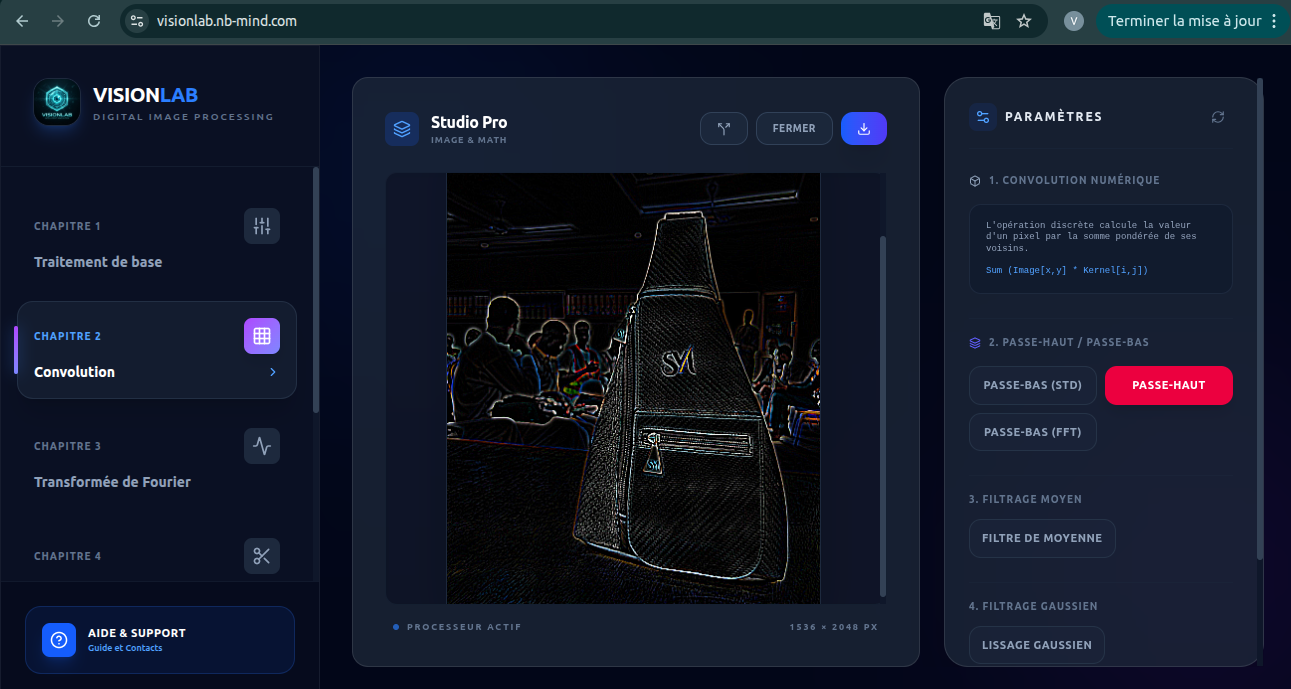
\includegraphics[width=\linewidth]{capture_ch2.png}
    \begin{tikzpicture}
      \fill[uy1blue!8, rounded corners=6pt] (0,0) rectangle (5,4.5);
      \node[text=uy1blue, font=\footnotesize\bfseries] at (2.5,3.8) {CAPTURE D'ÉCRAN};
      \node[text=gray, font=\scriptsize, text width=4cm, align=center] at (2.5,2) {Résultat filtre gaussien\\ou moyenneur appliqué\\à une image\\[6pt]\texttt{capture\_ch2.png}};
    \end{tikzpicture}
  \end{columns}
\end{frame}

% ======================================================================
\section{Chapitre 3 — Transformée de Fourier}
% ======================================================================

\begin{frame}{Chapitre 3 : Analyse Fréquentielle (FFT)}
  \begin{columns}[T]
    \column{0.52\textwidth}
    \begin{block}{Transformée de Fourier 2D Discrète}
      \[ F(u,v) = \sum_{x=0}^{M-1} \sum_{y=0}^{N-1} f(x,y)\, e^{-j2\pi\left(\frac{ux}{M} + \frac{vy}{N}\right)} \]
    \end{block}
    \vspace{4pt}
    \textbf{Implémentation :}
    \begin{itemize}
      \item Algorithme \textbf{Cooley-Tukey} (FFT~1D) appliqué ligne par ligne puis colonne par colonne
      \item Padding à la puissance de~2 supérieure
      \item \textbf{Spectre de magnitude} :
        $|F(u,v)| = \sqrt{\text{Re}^2 + \text{Im}^2}$
      \item Filtrage idéal :
        \begin{itemize}
          \item \textbf{Passe-bas} : $H(u,v) = 1$ si $D(u,v) < D_0$
          \item \textbf{Passe-haut} : $H(u,v) = 1$ si $D(u,v) > D_0$
        \end{itemize}
    \end{itemize}

    \column{0.45\textwidth}
    % ► CAPTURE : Spectre de Fourier ou résultat filtre FFT
    % 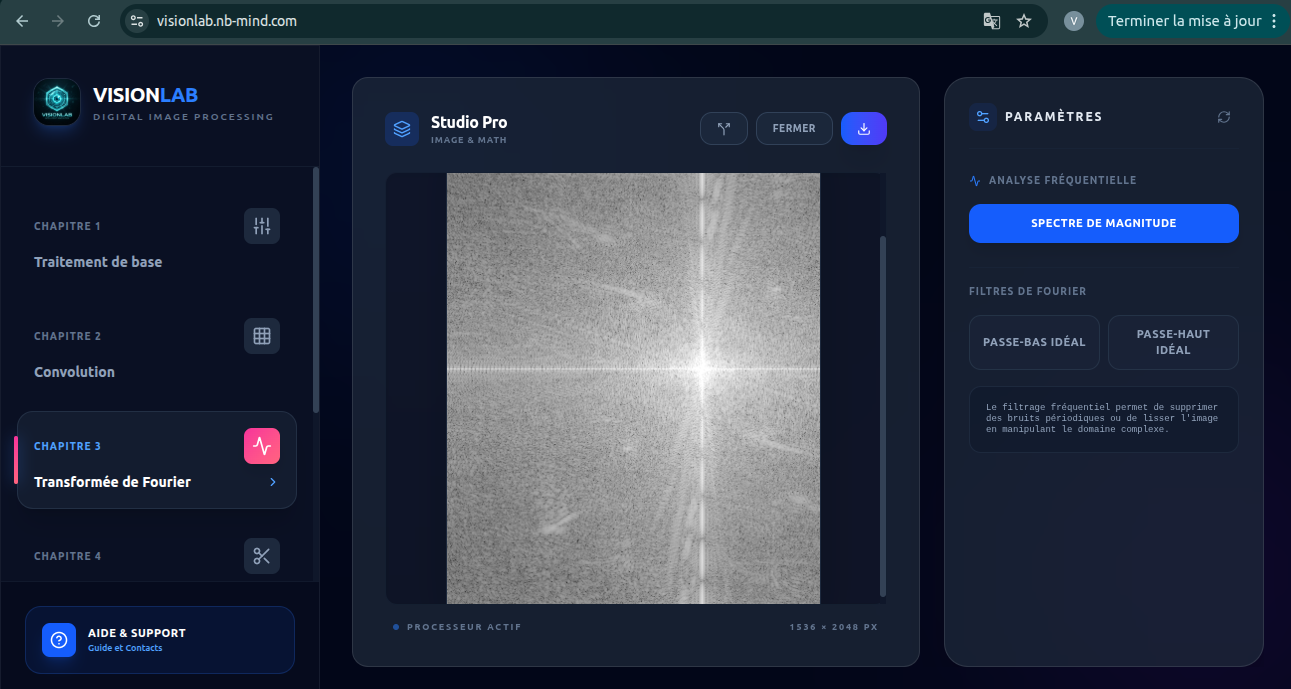
\includegraphics[width=\linewidth]{capture_ch3.png}
    \begin{tikzpicture}
      \fill[uy1blue!8, rounded corners=6pt] (0,0) rectangle (5,4.5);
      \node[text=uy1blue, font=\footnotesize\bfseries] at (2.5,3.8) {CAPTURE D'ÉCRAN};
      \node[text=gray, font=\scriptsize, text width=4cm, align=center] at (2.5,2) {Spectre de magnitude\\ou résultat du filtre\\passe-bas/haut idéal\\[6pt]\texttt{capture\_ch3.png}};
    \end{tikzpicture}
  \end{columns}
\end{frame}

% ======================================================================
\section{Chapitre 4 — Détection de Contours}
% ======================================================================

\begin{frame}{Chapitre 4 : Détection de Contours}
  \begin{columns}[T]
    \column{0.55\textwidth}
    \textbf{\textcolor{uy1blue}{Opérateurs implémentés :}}
    \vspace{4pt}

    \begin{tabular}{lcc}
      \toprule
      \textbf{Méthode} & \textbf{Type} & \textbf{Masque} \\
      \midrule
      Sobel & Gradient & $3 \times 3$ \\
      Prewitt & Gradient & $3 \times 3$ \\
      Robert & Gradient & $2 \times 2$ \\
      Isotrope & Gradient ($\sqrt{2}$) & $3 \times 3$ \\
      Laplacien & Dérivée 2\textsuperscript{nde} & $3 \times 3$ \\
      Gradient & Différences finies & $1 \times 2$ \\
      \bottomrule
    \end{tabular}
    \vspace{6pt}

    \begin{exampleblock}{Transformée de Hough}
      Détection de lignes droites par vote dans l'espace $(\rho, \theta)$ :
      \[ \rho = x\cos\theta + y\sin\theta \]
    \end{exampleblock}

    \column{0.42\textwidth}
    % ► CAPTURE : Résultat Sobel ou Hough
    % 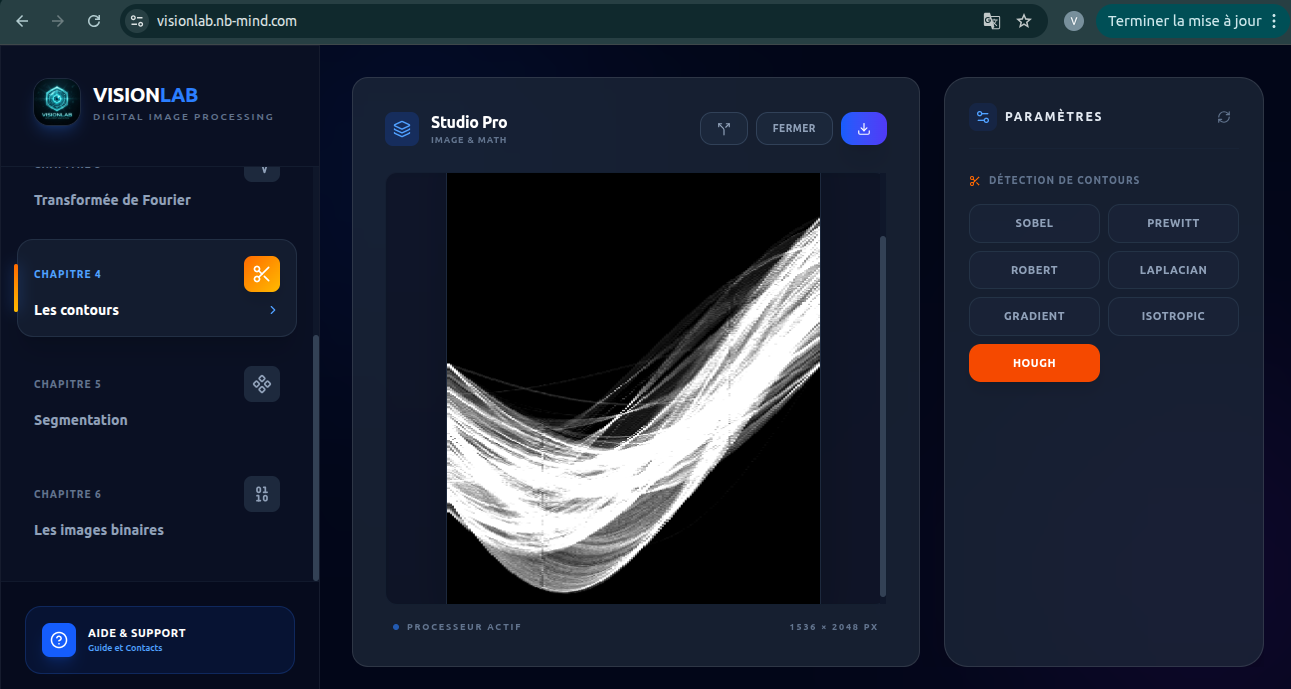
\includegraphics[width=\linewidth]{capture_ch4.png}
    \begin{tikzpicture}
      \fill[uy1blue!8, rounded corners=6pt] (0,0) rectangle (5,4.5);
      \node[text=uy1blue, font=\footnotesize\bfseries] at (2.5,3.8) {CAPTURE D'ÉCRAN};
      \node[text=gray, font=\scriptsize, text width=4cm, align=center] at (2.5,2) {Résultat Sobel / Prewitt\\ou espace de Hough\\[6pt]\texttt{capture\_ch4.png}};
    \end{tikzpicture}
  \end{columns}
\end{frame}

% ======================================================================
\section{Chapitre 5 — Segmentation}
% ======================================================================

\begin{frame}{Chapitre 5 : Segmentation par Seuillage}
  \begin{columns}[T]
    \column{0.52\textwidth}
    \begin{block}{Seuillage Manuel}
      \[ g(x,y) = \begin{cases} 255 & \text{si } f(x,y) \geq T \\ 0 & \text{sinon} \end{cases} \]
    \end{block}
    \vspace{4pt}
    \begin{block}{Méthode d'Otsu (Automatique)}
      Maximise la variance inter-classe :
      \[ \sigma_B^2(t) = w_0(t)\, w_1(t)\, [\mu_0(t) - \mu_1(t)]^2 \]
      Le seuil optimal $T^*$ est celui qui maximise $\sigma_B^2$.
    \end{block}
    \vspace{4pt}
    \begin{itemize}
      \item Curseur interactif pour le seuillage manuel
      \item Bouton dédié pour l'analyse automatique d'Otsu
    \end{itemize}

    \column{0.45\textwidth}
    % ► CAPTURE : Résultat segmentation (Otsu ou seuillage)
    % 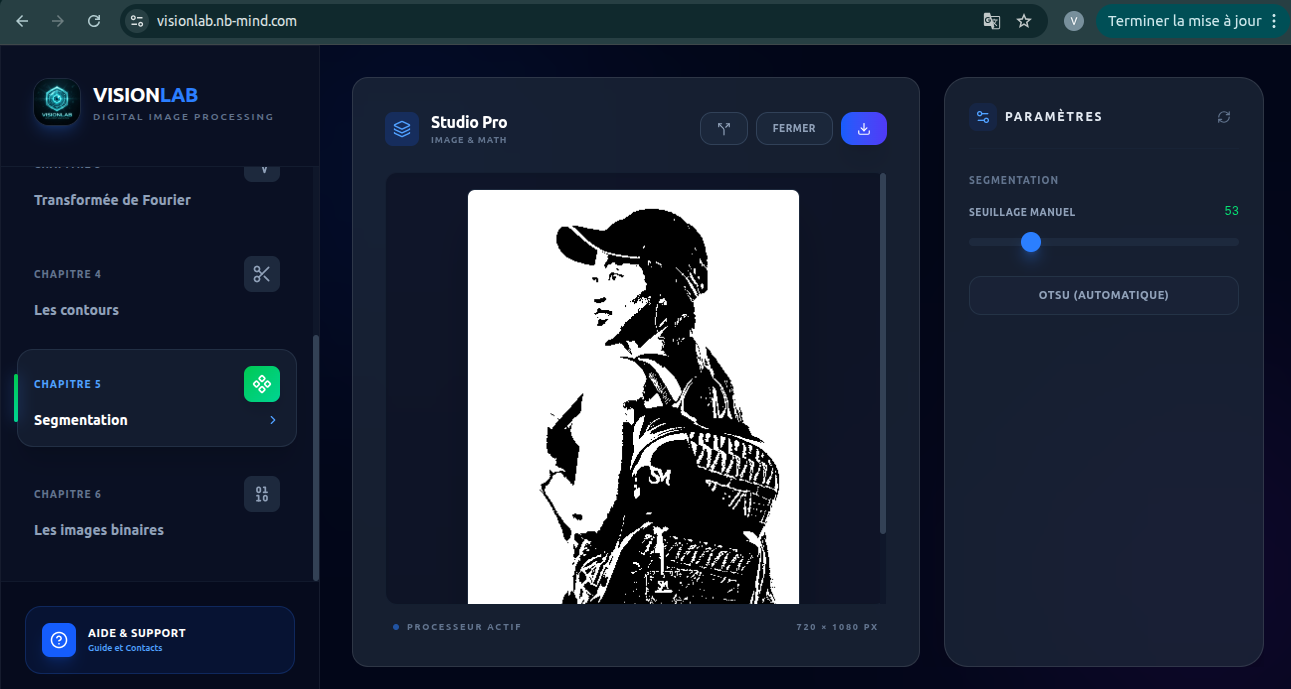
\includegraphics[width=\linewidth]{capture_ch5.png}
    \begin{tikzpicture}
      \fill[uy1blue!8, rounded corners=6pt] (0,0) rectangle (5,4.5);
      \node[text=uy1blue, font=\footnotesize\bfseries] at (2.5,3.8) {CAPTURE D'ÉCRAN};
      \node[text=gray, font=\scriptsize, text width=4cm, align=center] at (2.5,2) {Image binarisée\\par Otsu ou seuillage\\manuel\\[6pt]\texttt{capture\_ch5.png}};
    \end{tikzpicture}
  \end{columns}
\end{frame}

% ======================================================================
\section{Chapitre 6 — Morphologie Mathématique}
% ======================================================================

\begin{frame}{Chapitre 6 : Morphologie Mathématique}
  \begin{columns}[T]
    \column{0.52\textwidth}
    \textbf{\textcolor{uy1blue}{Opérations de base avec élément structurant $3\times 3$ :}}
    \vspace{4pt}
    \begin{itemize}
      \item \textbf{Érosion} : $E = A \ominus B = \{z \mid B_z \subseteq A\}$
      \item \textbf{Dilatation} : $D = A \oplus B = \{z \mid B_z \cap A \neq \emptyset\}$
    \end{itemize}
    \vspace{6pt}
    \textbf{\textcolor{uy1purple}{Opérations dérivées :}}
    \begin{itemize}
      \item \textbf{Ouverture} : $A \circ B = (A \ominus B) \oplus B$
      \item \textbf{Fermeture} : $A \bullet B = (A \oplus B) \ominus B$
      \item \textbf{Gradient interne} : $A - (A \ominus B)$
      \item \textbf{Gradient externe} : $(A \oplus B) - A$
    \end{itemize}

    \column{0.45\textwidth}
    % ► CAPTURE : Résultat morphologie (érosion/dilatation)
    % 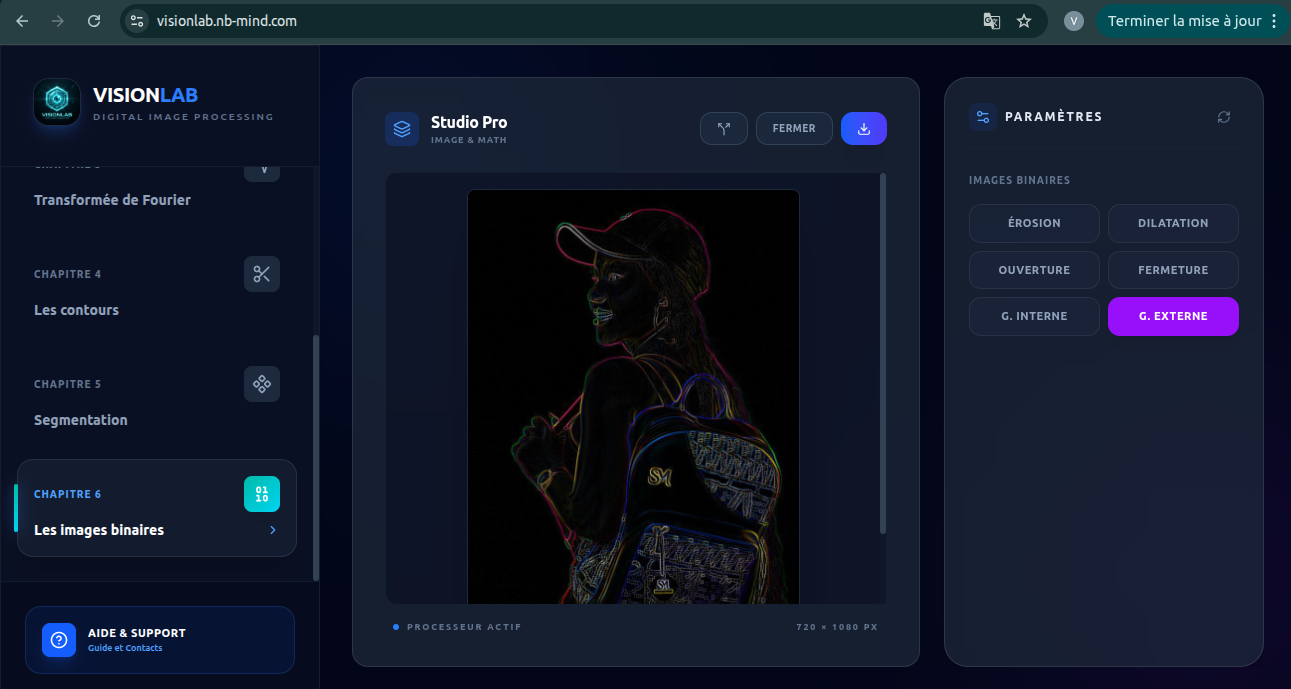
\includegraphics[width=\linewidth]{capture_ch6.png}
    \begin{tikzpicture}
      \fill[uy1blue!8, rounded corners=6pt] (0,0) rectangle (5,4.5);
      \node[text=uy1blue, font=\footnotesize\bfseries] at (2.5,3.8) {CAPTURE D'ÉCRAN};
      \node[text=gray, font=\scriptsize, text width=4cm, align=center] at (2.5,2) {Résultat érosion,\\dilatation ou\\gradient morphologique\\[6pt]\texttt{capture\_ch6.png}};
    \end{tikzpicture}
  \end{columns}
\end{frame}

% ======================================================================
\section{Interface Utilisateur}
% ======================================================================

\begin{frame}{Interface Utilisateur — Design Premium}
  \begin{columns}[T]
    \column{0.48\textwidth}
    \textbf{\textcolor{uy1blue}{Principes de Design :}}
    \begin{itemize}
      \item UI moderne : \textbf{Glassmorphism} + Dark Mode
      \item Barre latérale avec navigation par chapitres
      \item Boutons \textbf{Toggle} (clic = activer, re-clic = désactiver)
      \item Comparaison avant/après par slider interactif
      \item Histogramme temps réel (Chart.js)
      \item Matrice de pixels ($8\times8$) en surimpression
      \item Export haute résolution
    \end{itemize}
    \vspace{4pt}
    \begin{exampleblock}{Page de Support}
      Guide utilisateur interactif avec sections extensibles par chapitre, crédits académiques et formulaire de don.
    \end{exampleblock}

    \column{0.48\textwidth}
    % ► CAPTURE : Vue d'ensemble du Studio avec des filtres
    % 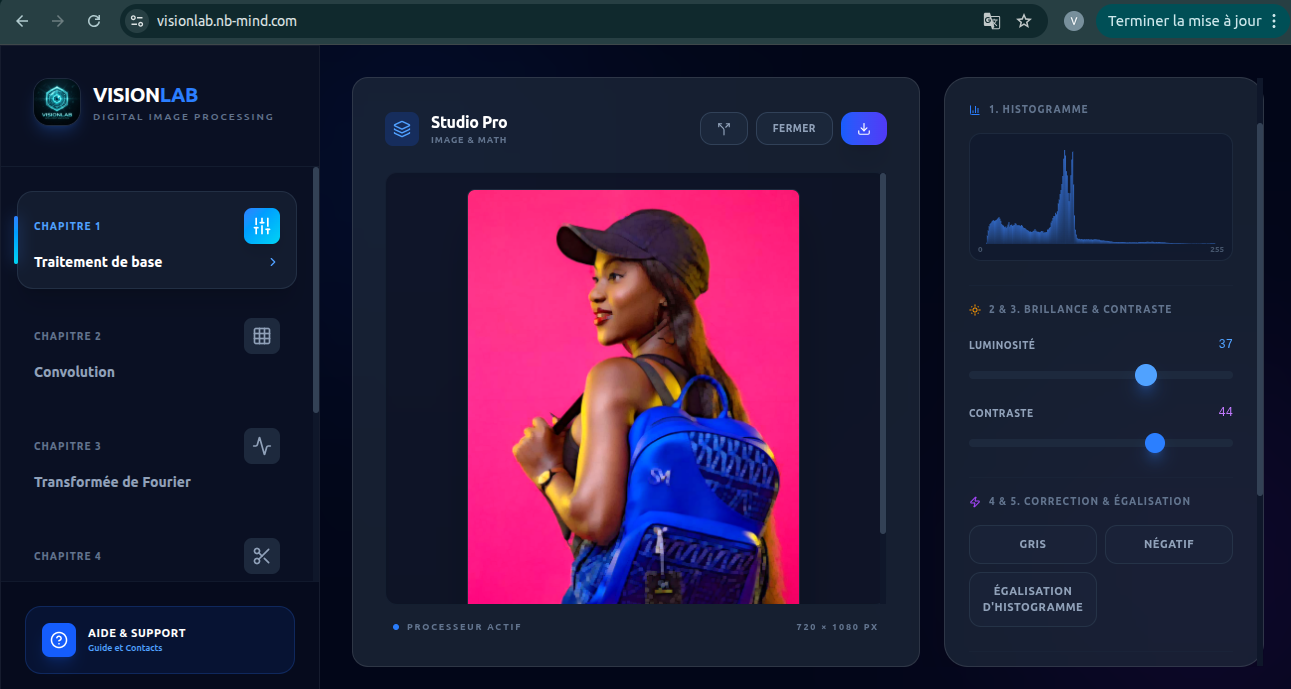
\includegraphics[width=\linewidth]{capture_studio.png}
    \begin{tikzpicture}
      \fill[uy1blue!8, rounded corners=6pt] (0,0) rectangle (5.5,4.8);
      \node[text=uy1blue, font=\footnotesize\bfseries] at (2.75,4.1) {CAPTURE D'ÉCRAN};
      \node[text=gray, font=\scriptsize, text width=4.5cm, align=center] at (2.75,2) {Vue d'ensemble du Studio\\avec sidebar + image traitée\\+ panneau de contrôle\\[6pt]\texttt{capture\_studio.png}};
    \end{tikzpicture}
  \end{columns}
\end{frame}

\begin{frame}{Page de Support \& Guide Utilisateur}
  \begin{columns}[T]
    \column{0.48\textwidth}
    % ► CAPTURE : Page Support (vue globale)
    % \includegraphics[width=\linewidth]{capture_support.png}
    \begin{tikzpicture}
      \fill[uy1blue!8, rounded corners=6pt] (0,0) rectangle (5.5,4);
      \node[text=uy1blue, font=\footnotesize\bfseries] at (2.75,3.3) {CAPTURE D'ÉCRAN};
      \node[text=gray, font=\scriptsize, text width=4.5cm, align=center] at (2.75,1.5) {Page Support :\\cartes des chapitres\\+ section contact\\[6pt]\texttt{capture\_support.png}};
    \end{tikzpicture}

    \column{0.48\textwidth}
    \textbf{\textcolor{uy1blue}{Contenu du Support :}}
    \begin{itemize}
      \item Guide interactif \textbf{6~chapitres}
      \item Bouton \og Voir plus \fg{} avec détails techniques et conseils d'utilisation
      \item Section \textbf{FAQ} intégrée
      \item Crédits académiques complets
      \item Formulaire de don avec popup de remerciement
      \item Contact : \texttt{visionlab.contacts@gmail.com}
    \end{itemize}
    \vspace{4pt}
    \begin{block}{Optimisation SEO}
      \footnotesize
      Balises meta (description, keywords, Open Graph), fichier \texttt{robots.txt}, titre optimisé pour l'indexation.
    \end{block}
  \end{columns}
\end{frame}

% ======================================================================
\section{Déploiement}
% ======================================================================

\begin{frame}{Déploiement et Mise en Ligne}
  \begin{center}
    \begin{tikzpicture}[
      box/.style={draw=uy1blue, fill=white, rounded corners=4pt,
                  minimum width=3.2cm, minimum height=1.2cm, font=\small\bfseries, align=center},
      arr/.style={->, very thick, uy1accent},
      scale=0.9, transform shape
    ]
      \node[box] (dev) at (0,0) {Code Source\\(VS Code)};
      \node[box] (git) at (5,0) {GitHub\\visionlab-git/\\visionlab};
      \node[box, fill=uy1green!10, draw=uy1green!60] (render) at (10,0) {Render\\(Static Site)};
      \node[box, fill=uy1purple!10, draw=uy1purple!50] (domain) at (10,-2.5) {Domaine\\personnalisé};

      \draw[arr] (dev) -- node[above, font=\scriptsize] {\texttt{git push}} (git);
      \draw[arr] (git) -- node[above, font=\scriptsize] {Auto-deploy} (render);
      \draw[arr, uy1purple] (render) -- node[right, font=\scriptsize] {CNAME DNS} (domain);

      \node[font=\footnotesize\bfseries, text=uy1green!80!black] at (10,-3.5) {\url{https://visionlab.nb-mind.com}};
    \end{tikzpicture}
  \end{center}
  \vspace{8pt}
  \begin{columns}[T]
    \column{0.48\textwidth}
    \begin{block}{Configuration Render}
      \footnotesize
      \begin{itemize}
        \item Root Directory : \texttt{frontend}
        \item Build : \texttt{npm install \&\& npm run build}
        \item Publish : \texttt{dist}
      \end{itemize}
    \end{block}
    \column{0.48\textwidth}
    \begin{block}{DNS Hostinger}
      \footnotesize
      \begin{itemize}
        \item Type : \texttt{CNAME}
        \item Name : \texttt{visionlab}
        \item Value : \texttt{visionlab-0s6x.onrender.com}
      \end{itemize}
    \end{block}
  \end{columns}
\end{frame}

% ======================================================================
\section{Conclusion}
% ======================================================================

\begin{frame}{Conclusion et Perspectives}
  \begin{columns}[T]
    \column{0.55\textwidth}
    \begin{exampleblock}{Réalisations Clés}
      \begin{itemize}
        \item[$\checkmark$] \textbf{6~chapitres} du cours entièrement implémentés
        \item[$\checkmark$] Interface \textbf{premium} et \textbf{responsive}
        \item[$\checkmark$] Pipeline de traitement \textbf{modulaire}
        \item[$\checkmark$] FFT~2D complète (Cooley-Tukey)
        \item[$\checkmark$] Déploiement avec domaine personnalisé
        \item[$\checkmark$] Documentation interactive intégrée
      \end{itemize}
    \end{exampleblock}
    \vspace{4pt}
    \begin{alertblock}{Perspectives}
      \begin{itemize}
        \item Web Workers pour les calculs lourds
        \item Intégration de la passerelle Mobile Money
        \item Ajout d'un chapitre \og Texture \fg{}
        \item Mode collaboratif en temps réel
      \end{itemize}
    \end{alertblock}

    \column{0.42\textwidth}
    \vfill
    \begin{center}
      \begin{tikzpicture}
        \fill[uy1blue!8, rounded corners=12pt] (-2.5,-2.8) rectangle (2.5,2.8);
        \node[font=\Large\bfseries, text=uy1blue] at (0,2) {Merci !};
        \draw[uy1accent, thick] (-1.5,1.5) -- (1.5,1.5);
        \node[font=\small, text=uy1dark, text width=4.2cm, align=center] at (0,0.5) {\textbf{NASSARAMADJI Nasaire}\\Licence~3 Informatique};
        \node[font=\footnotesize, text=gray, text width=4.2cm, align=center] at (0,-0.5) {Superviseur :\\Pr TAPAMO KENFACK\\Hippolyte};
        \draw[uy1accent, thick] (-1.5,-1.2) -- (1.5,-1.2);
        \node[font=\tiny, text=uy1accent] at (0,-1.7) {\url{https://visionlab.nb-mind.com}};
        \node[font=\tiny, text=gray] at (0,-2.2) {visionlab.contacts@gmail.com};
      \end{tikzpicture}
    \end{center}
    \vfill
  \end{columns}
\end{frame}

\end{document}
